\documentclass[11pt]{article}

\usepackage{amsmath}
\usepackage{amssymb}
\usepackage{titlesec}
\usepackage[utf8]{inputenc}
\usepackage[margin=2cm]{geometry}
\usepackage{prftree}
\usepackage{changepage}
\usepackage{enumitem}
\usepackage{minted}
\usepackage{graphicx}
\usepackage{wrapfig}

\title{\vspace{-2.5cm}CompArch\vspace{-2cm}}
\author{}
\date{}

\setlength{\parindent}{0cm}
\setlength{\parskip}{2mm}
\setlist{nosep}

% Make ~ look more normal
\let\oldsim\sim 
\renewcommand{\sim}{{\oldsim}}

\newminted[monospacefigure]{text}{linenos, frame=lines, framesep=1mm, autogobble, escapeinside=\#\#, mathescape, breaklines, xleftmargin=7mm}

\titlespacing{\section}{0mm}{2mm}{2mm}
\titlespacing{\subsection}{0mm}{2mm}{2mm}
\titlespacing{\subsubsection}{0mm}{2mm}{2mm}

\begin{document}
\maketitle

\section*{Design Metrics}
{ 
    \begin{minipage}[t]{0.3\textwidth}
    \begin{itemize}
    \item Energy
    \item Power
    \item Performance
    \item Security
    \item Cost
    \item Power Efficiency
    \item Reliability
    \end{itemize}
    \end{minipage}
    \begin{minipage}[t]{0.65\textwidth}
    \begin{itemize}
    \item Focus on common case: overall speed increases even if specific speed decreases.
    \item Amdahl's Law: \(\text{speedup} = \frac{1}{\text{sequential} + \frac{1 - \text{sequential}}{\text{speedup}_\text{enhanced}}}\)
    \item Adding enhancements means lower transistor budget, more localised heat, slower clock freq, .... Might affect common case.
    \item
    {
        \[\frac{1}{\text{performance}} = \frac{\text{time}}{\text{program}} = \frac{\text{instructions}}{\text{program}} \times \frac{\text{cycles}}{\text{instruction}} \times \frac{\text{time}}{\text{cycle}}\]

        \begin{itemize}
        \item Instruction count is affected by the ISA and compiler tech.
        \item CPI is affected by micro-architecture and ISA.
        \item Cycle time is affected by circuit design and micro-architecture.
        \end{itemize}
    }
    \end{itemize}
    \end{minipage}
}
\section*{ISAs}
{
    Each ISA is split into the System ISA and the User ISA. System ISA is privileged in some way.

    ISAs either break binary compatibility or carry architectural baggage. Embedded ISAs are more flexible as binary compatibility is less of an issue (mostly purpose-made binaries for product lifetime).

    Can use eg.\ JVM to remove reliance on specific ISA, or allow the processor to dynamically translate (Intel CISC-to-RISC).

    Microcode is code for running the ISA -- miniature control computer. Useful for CISC but introduces performance and complexity overhead.

    RISC ensures instructions are simple for faster fetching, easier pipelining. Relies on compiler to schedule and register-allocate.
}
\section*{Pipelining}
{
    \begin{center}
    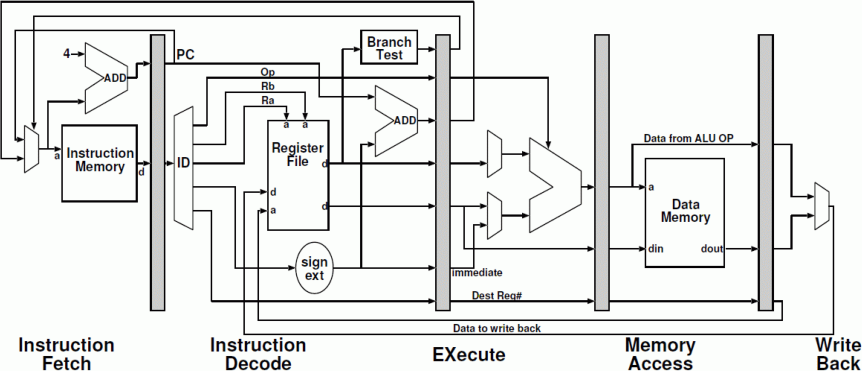
\includegraphics[width=0.8\textwidth]{pipeline.png}
    \end{center}

    \subsection*{Hazards}
    {
        Hazards are phenomena that require stalling in order to preserve program semantics.

        \begin{itemize}
        \item Structural Hazard (CPU resource conflicts, like limited ALU ports)
        \item Data Hazard (inter-instruction dependencies)
        \item Control Hazard (instructions changing the PC like \texttt{jmp})
        \end{itemize}

        \begin{minipage}[t]{0.7\textwidth}
        Instruction dependencies exist between \textbf{any} ordered pairs of instructions, regardless of distance, and make \textbf{reordering} harder.
        \begin{itemize}
        \item
        {
            True data dependence (result is truly required)
            \begin{itemize}
            \item \textbf{RAW}: 1 and 2.
            \end{itemize}
        }
        \item
        {
            Name dependence (same register used for multiple computations)
            \begin{itemize}
            \item \textbf{WAW}: 1 and 4.
            \item \textbf{WAR}: 2 and 3, 2 and 4.
            \end{itemize}
        }
        \end{itemize}
        \end{minipage}
        \begin{minipage}[t]{0.29\textwidth}
        \begin{monospacefigure}
        ADD R1, R2, R3
        SW  R1, 0(R4)
        SUB R4, R3, R5
        ADD R1, R2, R3
        \end{monospacefigure}
        \end{minipage}

        \textit{Structural hazards} can be avoided entirely in hardware/ISA (eg.\ avoid structural by having worst-case number of on-chip resources), but it can slow the common case or simply be too expensive. More complex but faster to handle issues as they come.

        \textit{Data hazards} can be avoided by adding data-forward paths, or scheduling code to prevent data dependencies from becoming data hazards (\textbf{instruction scheduling} by compiler/hardware). Hazards from name dependencies can be solved by \textbf{register renaming} (compiler/hardware).

        \begin{itemize}
        \item Software interlock: compiler inserts instructions on instructions causing a hazard.
        \item Hardware interlock: pipeline stalls when hazards are detected.
        \end{itemize}

        \textit{Control Hazards} can sometimes be avoided by branch prediction. In the simplest pipeline, just stall the fetches until the outcome of the branch is known. For simple tests (\(r = 0\)), could move test and target-address calculation into the decode stage. Requires dedicated hardware and logic for switching to, but reduces the branch delay slot by 1 cycle. Can embrace the branch delay slot and force compilers to place an instruction there.
    }
    \subsection*{Exceptions}
    {
        Page fault, illegal op-code, memory protection violation, arithmetic exception, I/O interrupt, ....

        Often want to be able to restart execution after handling the exception: a pipeline supports \textbf{precise exceptions} if it guarantees that all instructions prior to the faulting instruction have been executed and all those after it have not begun execution.

        Simple approach is to tag each instruction with its PC and a flag for whether it raised an exception. Execute stage sets the flag, and stages don't perform side-effects for instructions with the flag set. When the write-back stage sees a faulted instruction it flushes the pipeline.

        Alternatively, hand over control to dedicated hardware when an exception occurs (eg.\ for TLB misses) without flushing the pipeline.
    }
    \subsection*{Multicycle operations}
    {
        Not all instructions can/should complete in a single cycle (eg.\ floating point arithmetic, load/store operations).

        Use multiple execution pipelines, with all the issues arising there: new hazards, harder exception handling, etc.
    }
    \subsection*{Limits}
    {
        \begin{itemize}
        \item Deeper pipelines have more expensive stalls/flushes.
        \item Cycle time determined by worst-case stage time.
        \item Hard to clock each stage at the same time.
        \item More stages increases complexity (forwarding paths, harder exceptions, ...)
        \item Pipelining registers introduce overheads.
        \end{itemize}
    }
    \subsection*{Branch Prediction}
    {
        \begin{itemize}
        \item Condition codes: branch instructions have attached flags for the ALU (test against 0, allow overflow, ...)
        \item Condition registers: comparison operations store results in a given register, branches use those.
        \item Compare-and-branch: comparison and branch within a single instruction (Java bytecode).
        \end{itemize}

        \subsubsection*{Static Predictor}
        {
            Always guess `branch hit' or `branch miss'. Can improve results by allowing branch instructions to be tagged with a bias bit, that changes which way the processor guesses. Bit can be set by compiler, maybe using a profiling run to get an approximate distribution.
        }
        \subsubsection*{One-level Predictor}
        {
            Use a table of registers, indexed by a portion of the \textit{address of the branch}. 1 bit entries store taken/not taken. 2-bit entries can use a counter, to add a bit more consistency. Any more than 2 bits aren't much more effective.

            Don't care about collisions in the table as prediction is inaccurate anyway.
        }
        \subsubsection*{Two-level Predictor}
        {
            Local-history two-level predictors use a table of shift registers (history registers, like 01101) storing the branch's latest taken/not-takens. Also keep a table per branch, indexed by that branch's history register with entries being 2-bit counters like above.

            First level is the shift register holding a branch's history. Second level is using that history register to look up the prediction.

            Global history predictor uses a single shift register to hold the global history of branches, rather than a specific hash of them. Second level is the same, just the first level is less interesting.

            \textit{Check in supo notes that Daniel agreed with the global predictor definition.}
        }
        \subsubsection*{Tournament Predictor}
        {
            Local and Global predictors are effective in different cases. Use both, and pick whichever has been most accurate for a specific branch in the past.
        }
        \subsubsection*{Limits}
        {
            \begin{itemize}
            \item Need a training period of low accuracy before predictors get up to speed.
            \item Will always be malicious inputs.
            \item Can be very expensive to implement (two big tables for each branch...)
            \item Using hashing on the branch PC, so can have negative/positive/neutral aliasing of branches.
            \end{itemize}
        }
        \subsubsection*{Branch Target Buffer/\textbf{Cache}}
        {
            \begin{minipage}[t]{0.7\textwidth}
            \vspace{0pt}
            As well as predicting whether a branch will be taken, can also predict where it'll go: if we predict it being taken, save time working out the destination.

            Keep a table indexed by the branch address with entries being cached target addresses.

            All this happens during instruction fetch, so if we guess correctly on branch prediction and the cached value is correct, we don't incur \textbf{any} branch penalty.
            \end{minipage}
            \begin{minipage}[t]{0.29\textwidth}
            \vspace{0pt}
            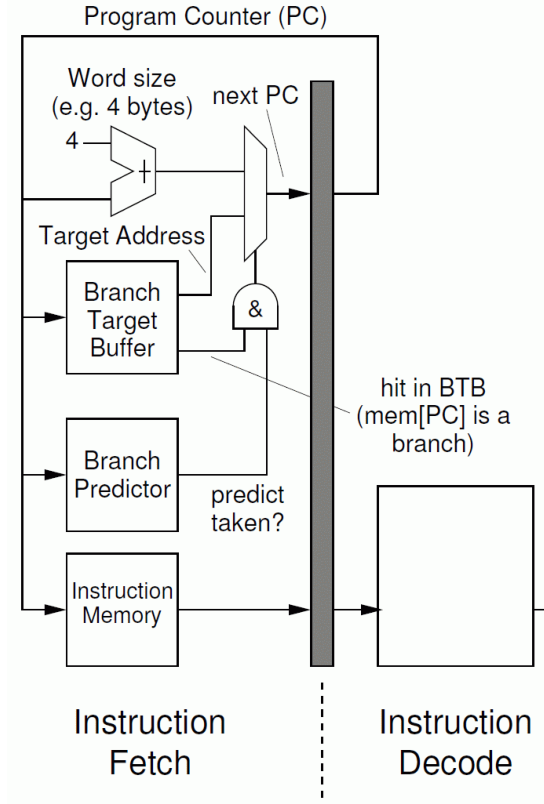
\includegraphics[width=\textwidth]{btb.png}
            \end{minipage}
        }
        \subsubsection*{Return Address Predictors}
        {
            Functions can be called from all over the place so predictions are normally inaccurate.

            Just store a stack of PCs from before branches.
        }
        \subsubsection*{Avoiding Branches}
        {
            ARM conditional instructions allow transforming control dependencies (branches) into data dependencies (normal instructions with conditional flags). End up with nullified pipeline instructions but will never have to flush the pipeline. Only works for simple branches where it's worth inlining. In the end, branch prediction is just accurate enough that this is unnecessary.
        }
    }
}
\section*{Superscalar Processors}
{
    Exploit instruction-level parallelism (ILP) to replace stalls with instructions.

    \subsection*{Superpipelined}
    {
        Further subdivide pipeline macro-stages into \(M\) micro-stages that \textbf{all do the same thing}: each clock allows for \(M\) instructions to complete.

        \textit{Check supo notes for why superparallel isn't used.}

        Reminder that pipeline stages can be divided as far as we want: the 5-stage pipeline is human-friendly but each stage can be divided into subtasks arbitrarily.
    }
    \subsection*{Superscalar}
    {
        \begin{center}
        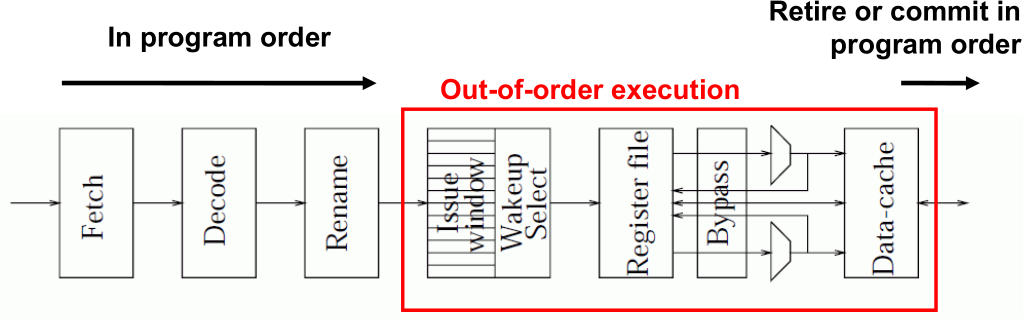
\includegraphics[width=0.8\textwidth]{out-of-order.png}
        \end{center}

        Run \(P\) pipelines in parallel. \(\text{IPC} \leq P\), clock period stays the same as in a pipelined processor.

        Upper limit on ILP is due to true data dependencies. Can exceed even this by using special multi-input or extra-fast functional units to run multiple cheap instructions within a cycle (eg.\ \texttt{ADD}).

        \textbf{Processor can't sustain an execution rate faster than the fetch rate}.

        \subsubsection*{Fetch Techniques}
        {
            Need multi-ported instruction caches for fetching up to \(P\) instructions per cycle. Can be complex if the instructions don't \textbf{align} with the cache lines (eg.\ we fetch 4 instructions starting from 2 when the cache lines start from 0, 4, ...).
        }
        \subsubsection*{Register Renaming}
        {
            Can reduce the effects of name dependencies (using the same register) by having a large set of \textbf{physical registers} which are mapped onto by the \textbf{architectural registers} which are exposed to the program.

            The rename stage keeps a list of free registers and the current mapping from architectural to physical registers and rewrites instructions just before they enter the out-of-order portion of the pipeline.
            
            Output registers are \textbf{always renamed}, as otherwise we're not actually helping hide name dependencies. Essentially rewrites into SSA form.
        }
        \subsubsection*{Out-of-order execution}
        {
            Compiler is often unable to schedule instructions optimally as it can't disambiguate memory addresses, can't predict branches, works with a limited number of registers.

            Maintain a buffer of instructions waiting to execute. Issue instructions from the buffer in any order once they're ready to execute (all operands are available and a functional unit is free).

            When an instruction is scheduled, its destination register is marked as ready for during the next cycle, so subsequent instructions can get scheduled.

            Usually want to schedule loads as early as possible, as they take a long time and often free up lots of other instructions.

            \begin{itemize}
            \item Load Bypassing: execute loads before stores \textbf{if they access different memory locations}.
            \item Store-to-Load Forwarding: if a load reads from the same location as a store, just forward the stored value to the load instruction -- completely skip memory read.
            \item Load-to-Load Forwarding: forward data from an earlier read to a later one.
            \end{itemize}
        }
        \subsubsection*{Load/Store Queues}
        {
            \begin{wrapfigure}{R}{0.4\textwidth}
            \centering
            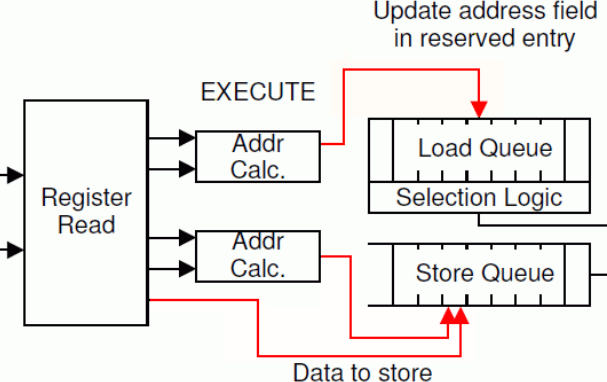
\includegraphics[width=0.35\textwidth]{load-store-queues.png}
            \end{wrapfigure}
            Inbetween execute and memory access, keep two queues for load/store instructions. Each queue is in program order, indexed by the instruction address and containing the instruction. Operands might not have been calculated (queue could contain \texttt{4: STORE 3 0x...} and \texttt{5: STORE 4 ?}, where \texttt{?} will get updated when the out-of-order address calculation happens).

            Stores can't be undone, so need to ensure that exceptions from earlier instructions are handled before performing a store, as well as that any speculation (of data or branch) has been confirmed.

            \begin{itemize}
            \item Always execute store instructions in program order: never reorder. Ensures that exceptions and mispredicted branches are handled.
            \item Before performing a load (moving it out of the load queue), search the store queue for a store to the same memory location. If there's a matching (youngest) store, skip the memory read and just use the value that's going to be stored (store-to-load forwarding). Stores might not have addresses calculated, so we need to treat loads as speculative (might get rolled back later).
            \item When a store address is calculated, update the instruction in the store queue and search the load queue for speculative loads to the same address -- need to roll them back.
            \end{itemize}

            Load/Store Queues are expensive as they compare wide memory addresses and need to be content-addressable, and usually multi-ported.
        }
        \subsubsection*{Avoiding Load/Store Queues}
        {
            Alternate approach: disallow store-to-load forwarding, and just flush the pipeline when out-of-order store/load instructions are detected to have been performed out of order.

            Use a hash table of counters indexed by accessed addresses to detect problems: increment the counter when a load is issued and decrement it on commit. If a store commits and the counter is non-zero, flush and restart the pipeline.
        }
    }
    \subsection*{Precise Exceptions and Rollbacks}
    {
        Exceptions are detected when processing one instruction in the instruction window, some of which have been performed and some not. Should only allow commits if no potential for an exception.

        \subsubsection*{The Reorder Buffer}
        {
            Keep an array of \textbf{register results} (not instructions) at the end of the pipeline in program order, the relevant slot being updated when an instruction executes. When all earlier instructions have completed, commit the results to the architectural register file.

            When committing, if we detect a mispredicted branch or exception we just clear the reorder buffer and restart the pipeline.

            Now have \textbf{two locations} for register contents: when an instruction uses operands, need to look in the reorder buffer for the youngest change to the register, and if it's not present, fall back to the real architectural register file.
        }
        \subsubsection*{Unified Register File}
        {
            \begin{wrapfigure}{R}{0.4\textwidth}
            \centering
            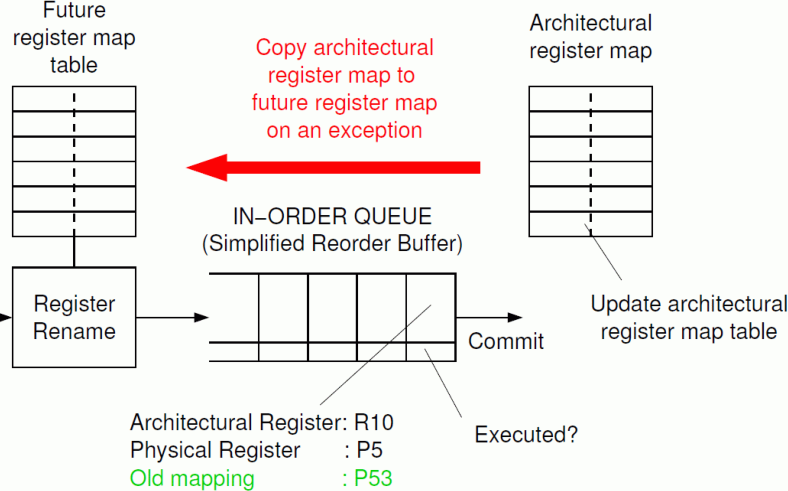
\includegraphics[width=0.4\textwidth]{unified-register-file.png}
            \end{wrapfigure}

            Use a single large register files instead of an auxiliary buffer, and use two mapping tables: each table is the state of a register-renaming.

            \begin{itemize}
            \item Front-end table is used by all running instructions and provides the latest speculative register values.
            \item Back-end table is the correct, committed mapping.
            \end{itemize}

            When there's an exception or misprediction, can just directly copy the back-end table over the front-end table to replace the speculative registers.

            Need an in-order queue representing instructions, holding the architectural and physical registers, as well as the old physical register for freeing up.
        }
    }
    \subsection*{Limits}
    {
        Diminishing returns from exploiting ILP when pipelines get wide. Complexity of the pipeline multiplied, so harder to optimise and verify.

        Requires high instruction fetch rate, imposes knock-on performance requirements on other components. Still centralised, so doesn't scale well.
    }
}
\section*{VLIW}
{
    \textbf{Very Large Instruction Width} processors move the scheduling complexity out of the processor and into the compiler.

    Idea is to use an ISA which supports packing a number of independent instructions into a single long instruction. Each slot in the instruction has a fixed function (integer op, load/store, floating-point, ...).

    Latency subtleties come into play: operations have different durations, so the compiler is forced to assume worst-case delay for each (assume eg. 3 instruction delay before memory ops are completed). If an operation takes longer (cache miss), the pipeline is just stalled.

    \subsection*{Local Scheduling}
    {
        \begin{wrapfigure}{R}{0.4\textwidth}
        \centering
        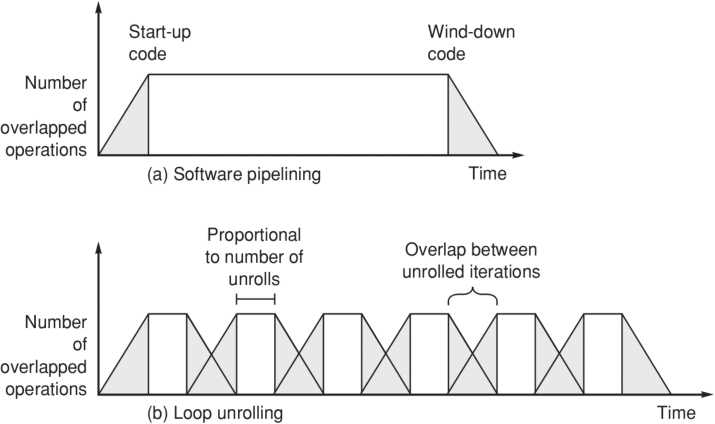
\includegraphics[width=0.37\textwidth]{software-pipelining.png}
        \end{wrapfigure}

        Scheduling within a basic block has limited ILP (less than 2 normally). Basic blocks are typically 5 instructions long (branch every 5 instructions).

        \subsubsection*{Loop Unrolling}
        {
            Replicate the loop body multiple times and change the loop condition to match. Adjust memory access offsets to account for being in a different block. Increases the size of the basic block in the loop body, so higher ILP inside the body.

            Requires some setup/teardown where there's very limited ILP (eg.\ need to load/store values before starting/finishing and there's no non-memory operations we can do in the meantime).
        }
        \subsubsection*{Software Pipelining}
        {
            Overlap different iterations of the loop so that we avoid the setup/teardown associated with loop unrolling. Each VLIW instruction has a slot filled by each iteration.

            Register renaming can get difficult if we need a result computed by an old iteration, as the register will get overwritten.

            \begin{itemize}
            \item Can add explicit register moves to store the results we need.
            \item Can do unrolling first, to make the kernel larger and bring the result into scope.
            \item Use a \textbf{Rotating Register File}: each iteration of the loop gets a fresh set of registers.
            \end{itemize}
        }
    }
    \subsection*{Global Scheduling}
    {
        Can move instructions between basic blocks to increase ILP, but it's complex: the state space is huge and finding an approximately optimal solution is expensive.

        \subsubsection*{Trace Scheduling}
        {
            \begin{minipage}[t]{0.55\textwidth}
            Focus on the common case: find the most likely \textbf{path} through the basic block graph using eg.\ annotated code/profiling, and name it the \textbf{trace}.

            The trace has side entrances and exits, caused by branches of other paths leading into the most probable one or branches moving us off the trace.

            Can optimise instruction layout within the trace rather than globally, then insert book-keeping instructions to compensate for the code motion when we move into/out of the trace. Moving in and out is expensive, but following the trace directly has a very high ILP.
            \end{minipage}
            \hspace{5mm}
            \begin{minipage}[t]{0.4\textwidth}
            \vspace{0pt}
            \centering
            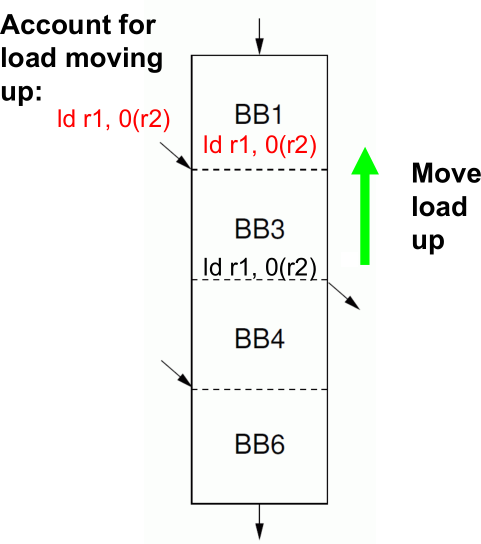
\includegraphics[width=\textwidth]{trace-scheduling.png}
            \end{minipage}
        }
    }
    \subsection*{Conditional Instructions}
    {
        Conditional instructions are effective for VLIW as they can fill slots in instructions that would otherwise be blank, even if they don't end up being executed.
    }
}
\section*{Multithreaded Processors: \textbf{Concurrency}}
{
    \begin{wrapfigure}{R}{0.6\textwidth}
    \centering
    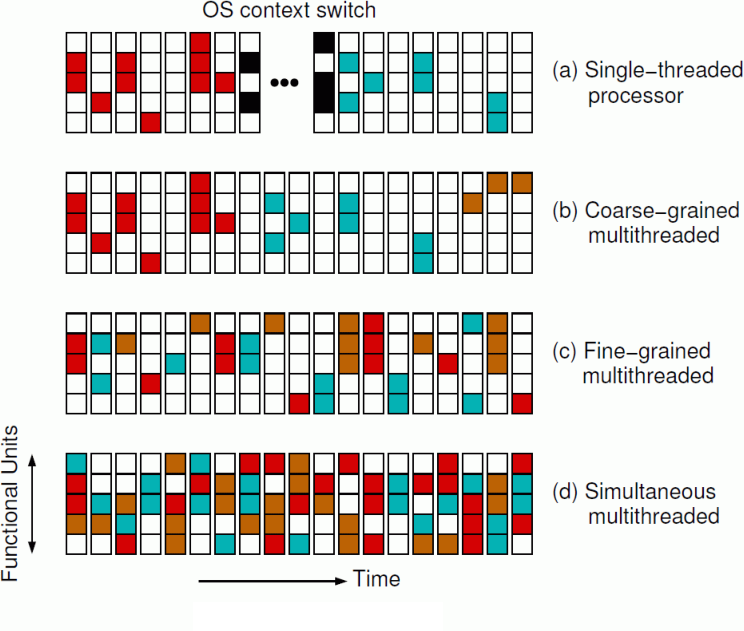
\includegraphics[width=0.57\textwidth]{multithreading-summary.png}
    \end{wrapfigure}
    
    Not parallelism, just running multiple threads on the same core. Often care about throughput over performance of a single thread, ie.\ in server workloads.

    ILP is relatively fine-grained parallelism: ensuring we get maximal throughput of instructions. TLP is coarser, based on independent workloads.

    \subsection*{Coarse-grained Multithreading}
    {
        Switch to an alternative thread when the active thread stalls (cache miss, IO, ...). Aim is to hide cache miss penalties and maintain higher utilisation.

        On a switch, we flush the pipeline, store any state, reload the new state, and start fetching new instructions. Need to ensure side-effects of currently executing instructions are either saved or rolled back.

        \begin{itemize}
        \item Shorter pipelines reduce thread switch penalty, as we don't need to refill the pipeline as much.
        \item Can use a \textbf{thread-switch buffer} to store a few instructions from each thread to avoid instruction cache misses. 
        \item \textbf{Pipeline registers} on each pipeline stage can hold in-execution state for a few threads at a time, then swap them in and out of the main pipeline quickly. Prevents the need to refill the pipeline.
        \end{itemize}
    }
    \subsection*{Fine-grained Multithreading}
    {
        A new thread is selected on each clock cycle: different instructions in the pipeline belong to different threads. Use eg.\ round robin to select threads.

        Static thread schedules can be wasteful if there aren't many threads, but can simplify dependency-handling logic: if we know the spacing between each thread, we can remove eg.\ data-forwarding.

        Fine-grained multiprocessors without caches can provide strict and predictable performance guarantees, compared to a pipeline processor with caches and coarse thread-switching.

        Can use dynamic thread-selection policies, or avoid switching to stalled threads, etc.
    }
    \subsection*{Simultaneous Multithreading}
    {
        Superscalar processors with multithreading and out-of-order execution can allow for instructions from different threads to be in-flight simultaneously.
    }
}
\section*{Caches}
{
    \begin{minipage}[t]{0.4\textwidth}
    Can use software-controlled caches/scratchpads for realtime systems, or hardware managed caches. Smaller is faster.

    Unified cache is data+instructions combined (level 2+), level 1 is separated caches. Separated isn't just faster, also means \textbf{can access instructions and data at the same time}.

    \textbf{Block = Cache Line}

    \subsection*{Direct Mapped Cache}
    {
        Each block can only live in one place in the cache: the block address `mod' the number of blocks in the cache. Fast, but suffers from collisions: cache lines are evicted even when there are free entries.

        Middle bits (index) are used as index into the cache. Low bits (offset) are used as cache line index. High bits (tag) are used to check for validity.
    }
    \end{minipage}
    \hspace{5mm}
    \begin{minipage}[t]{0.55\textwidth}
    \vspace{0pt}
    \centering
    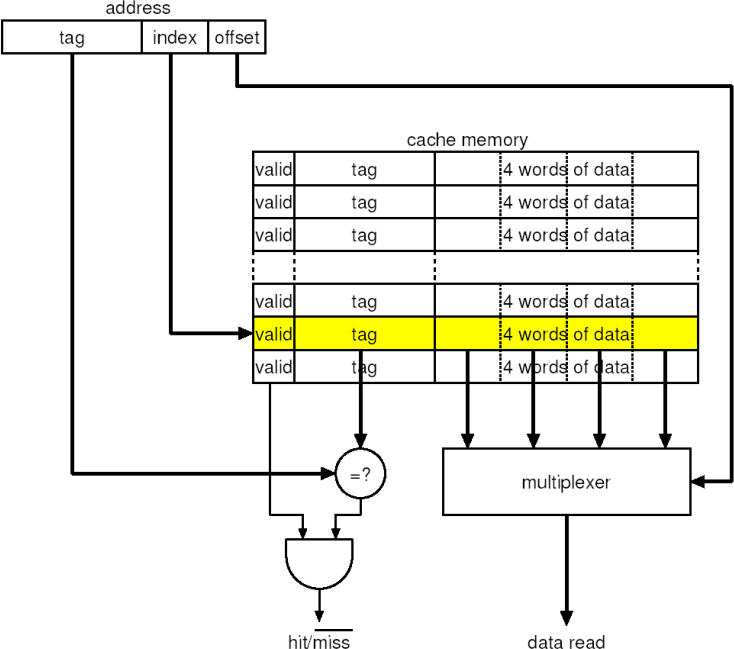
\includegraphics[width=\textwidth]{direct-cache.png}
    \end{minipage}
    \subsection*{Set Associative}
    {
        For an \(n\)-way set associative cache, store \(n\) sets/ways of blocks, each set/way being addressable by the index. Look up the line in all ways at the same time, and report whichever holds it.

        Can be the fastest type of cache.
    }
    \subsection*{Fully Associative Cache}
    {
        Can further divide memory into ways to get a highly- or fully-associative cache, but it's inefficient.

        Content Addressable Memories return addresses of data given the data.
    }
    \subsection*{Block Replacement}
    {
        Always replace blocks in a direct-mapped cache, but set-associative and fully associative need policies.

        Least Recently Used takes advantage of temporal locality, but can be expensive to implement. Random performs well on average, approximate LRU schemes exist.
    }
    \subsection*{Write Policies}
    {
        \begin{itemize}
        \item Write Through: write to cache and higher-level memory.
        \item Write Back: only write modified cache blocks when they're evicted.
        \end{itemize}

        If data isn't in the cache when we write to a memory address:
        \begin{itemize}
        \item Allocate Write: read the data into cache, then overwrite it.
        \item No Allocate Write: don't load lines to the store (lines are only loaded on a read miss).
        \end{itemize}

        Usually write-through + allocate-write and write-back + no-allocate-write.

        Inclusive caches ensure that addresses in higher-level memory are a superset of address in lower-level memory. Exclusive caches don't enforce this.
    }
    \subsection*{Cache Misses}
    {
        The three reasons for cache misses (the three C's):

        \begin{itemize}
        \item \textbf{Compulsory}: A compulsory miss happens when a block is brought into the cache for the first time.
        \item \textbf{Capacity}: A capacity miss occurs when the number of blocks exceeds the capacity of the cache.
        \item \textbf{Conflict}: Direct mapped and set-associative caches suffer conflict misses on collisions.
        \end{itemize}
    }
    % pg346
}
\end{document}